\documentclass[a4paper, pagesize, parskip=half]{scrartcl}

\usepackage[utf8]{inputenc}
\usepackage[T1]{fontenc}
\usepackage[english]{babel}

\usepackage{graphicx}

\usepackage[expansion=false, tracking=false, protrusion=true]{microtype}


\addtokomafont{disposition}{\rmfamily}
\renewcommand{\descfont}{\bf \rmfamily}

\begin{document}

\Huge \textbf{\textsc{Assignment 1}: Database Design}

\Large \textbf{Database Design I} \quad \large \today

\normalsize Group 4: \quad Björk, Alve  \quad Engström, Per \quad Orim, Paul \\*
\rule{\textwidth}{1pt}

\bigskip

\section*{Business logic}

\begin{itemize}
    \item \emph{Bibliography.Volume} is either the volume number if \emph{Bibliography.Periodical} is a journal, and otherwise an abbreviation of the publication type.
    
    \item \emph{Bibcode}s reference existing bibliography items.
    
    \item \emph{Object\_type}s must belong to the set of predefined types. \emph{Object\_type}s discriminate between \emph{Star} and \emph{Galaxy} entities.
    
    \item The \emph{Cross\_reference} should be a strict partial order.
    
    \item All data should follow the specification of SIMBAD.
\end{itemize}

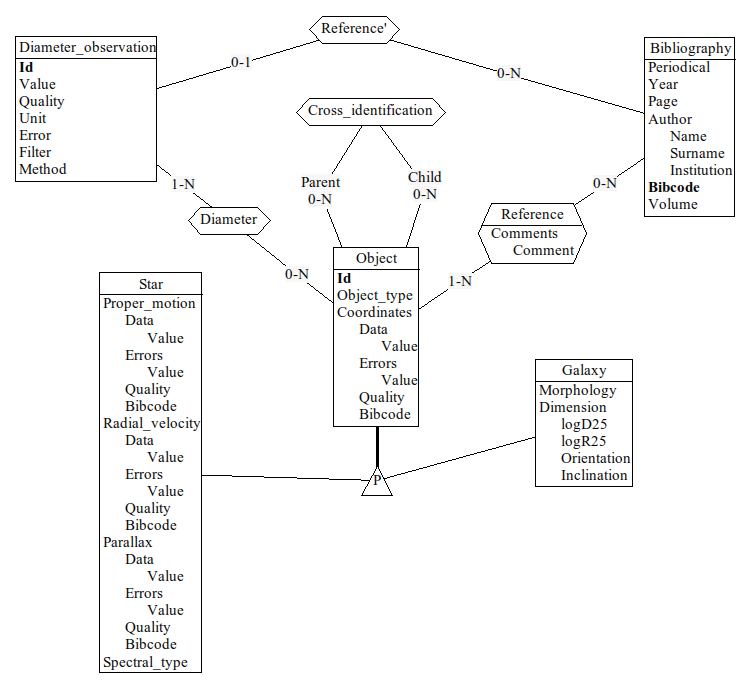
\includegraphics[width=\textwidth]{diagram.png}

\end{document}